% Generado por population_calibration.py
\begin{frame}[c]{Calibración poblacional: capa A}
  \centering
  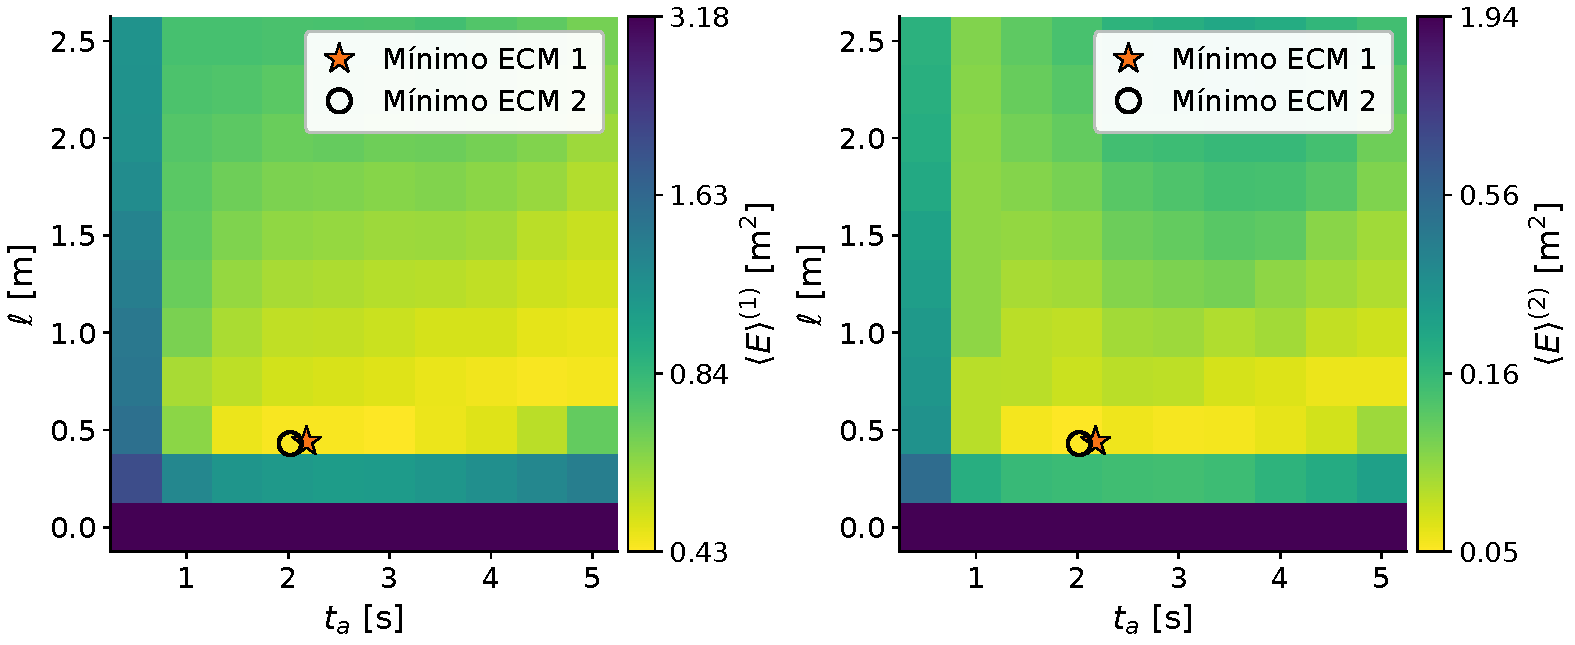
\includegraphics[width=\textwidth,height=4.4cm,keepaspectratio]{figuras/calibracion-A-mapas.pdf}
  \par\vspace{2mm}
  {\footnotesize\renewcommand{\arraystretch}{1.15}
  \begin{tabular}{@{}lccc@{}}
    \hline Criterio & $(p_1^*,p_2^*)$ & ECM 1 (m$^2$) & ECM 2 (m$^2$) \\ \hline
    \rowcolor{yellow!35} ECM 1 & $(2{,}18;\ 0{,}44)$ & $0{,}42289$ & $0{,}04137$ \\
ECM 2 & $(2{,}02;\ 0{,}43)$ & $0{,}42426$ & $0{,}04126$ \\
    \hline
  \end{tabular}\par}
\end{frame}

\begin{frame}[c]{Calibración poblacional: capa B}
  \centering
  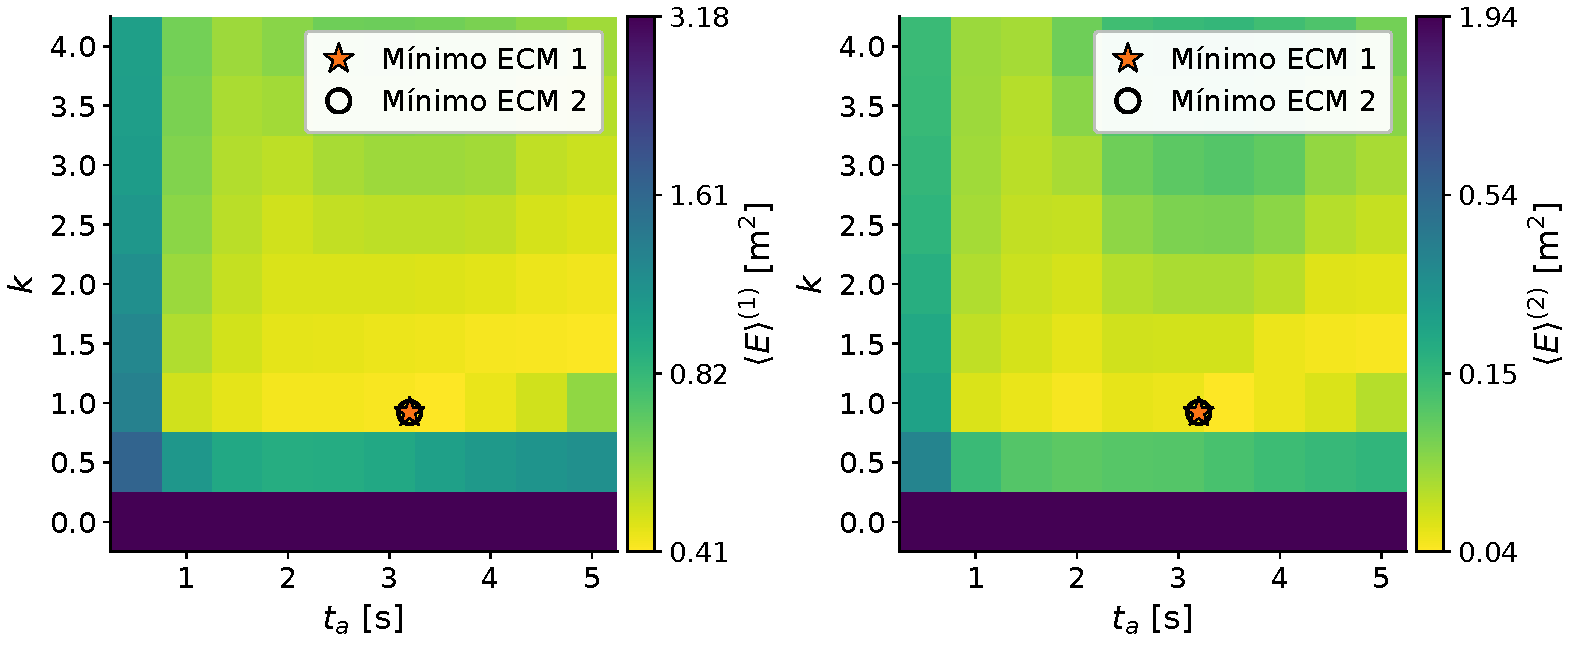
\includegraphics[width=\textwidth,height=4.4cm,keepaspectratio]{figuras/calibracion-B-mapas.pdf}
  \par\vspace{2mm}
  {\footnotesize\renewcommand{\arraystretch}{1.15}
  \begin{tabular}{@{}lccc@{}}
    \hline Criterio & $(p_1^*,p_2^*)$ & ECM 1 (m$^2$) & ECM 2 (m$^2$) \\ \hline
    \rowcolor{yellow!35} ECM 1 & $(3{,}2;\ 0{,}92)$ & $0{,}41144$ & $0{,}03982$ \\
ECM 2 & $(3{,}2;\ 0{,}92)$ & $0{,}41144$ & $0{,}03982$ \\
    \hline
  \end{tabular}\par}
\end{frame}

\begin{frame}[c]{Calibración poblacional: capa E}
  \centering
  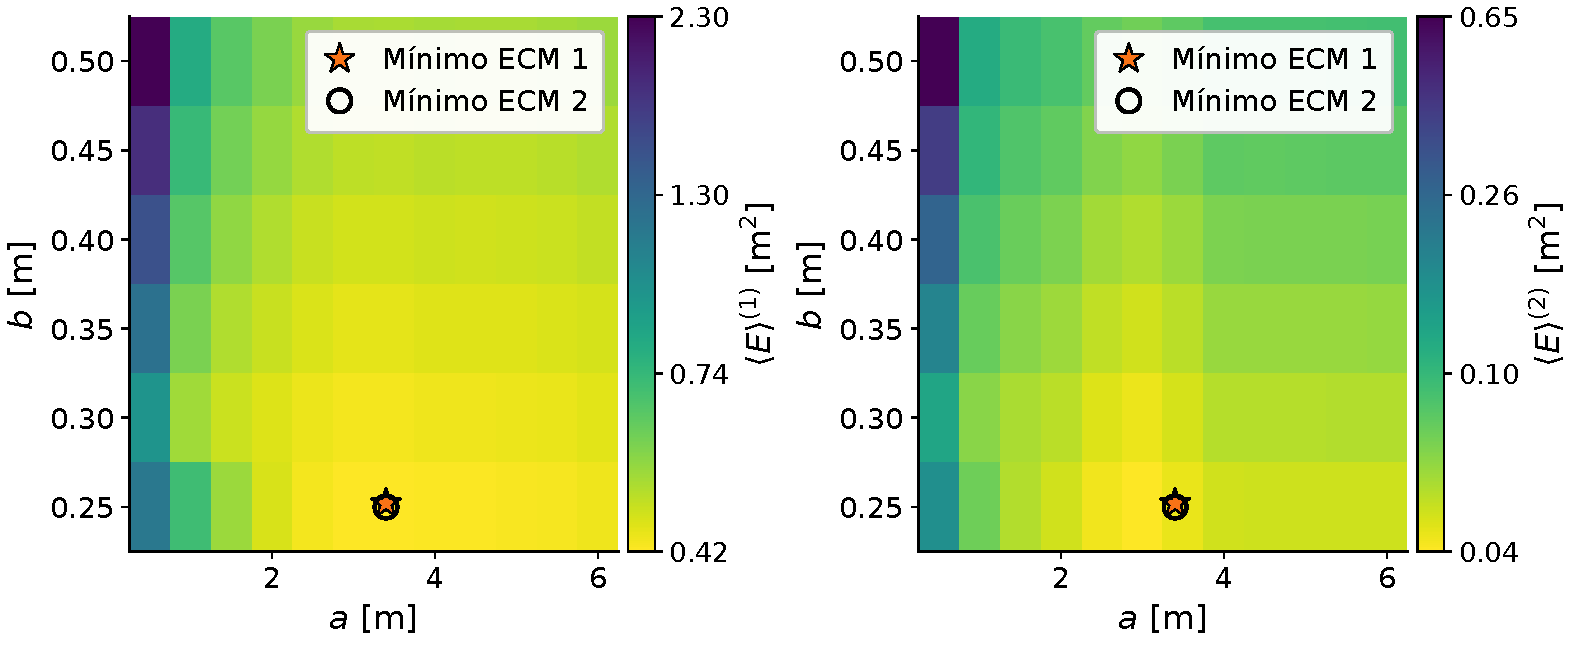
\includegraphics[width=\textwidth,height=4.4cm,keepaspectratio]{figuras/calibracion-E-mapas.pdf}
  \par\vspace{2mm}
  {\footnotesize\renewcommand{\arraystretch}{1.15}
  \begin{tabular}{@{}lccc@{}}
    \hline Criterio & $(p_1^*,p_2^*)$ & ECM 1 (m$^2$) & ECM 2 (m$^2$) \\ \hline
    ECM 1 & $(3{,}4;\ 0{,}252)$ & $0{,}40833$ & $0{,}03482$ \\
\rowcolor{yellow!35} ECM 2 & $(3{,}4;\ 0{,}25)$ & $0{,}40856$ & $0{,}03476$ \\
    \hline
  \end{tabular}\par}
\end{frame}
